% -----------------------------------------------------------------------------
%   Arquivo: ./02-elementos-textuais/resultados.tex
% -----------------------------------------------------------------------------

\begin{comment}

-- escrever um esquema dos experimentos que devem ser executados

-- separar em seções, uma pra cada experimento, apresentar o experimento, o resultado, e discutir

-- mostrar se o mecanismo funciona exatamente como esperado, para uma única criatura, as duas implementação são qualitativamente comparáveis 

-- estudar mais de uma criatura, mostrando que uma tem comportamento similar a outra, 


-- ARREFECIDA
\end{comment}


\chapter{Análise e Discussão dos Resultados}
\label{chap:resultados}
Apresentada no capítulo \autoref{chap:metodologia} a modelagem de um simulador de criaturas artificiais assíncrono e distribuído, baseado no arquitetura Artífice, é necessário validar dois aspectos do software proposto. Primeiro, no que diz respeito ao comportamento das criaturas artificiais, se ele é qualitativamente comparável com a arquitetura Artífice. O segundo aspecto a se verificar é quão escalável é o sistema, horizontal e verticalmente. Neste sentido, foram propostos três experimentos preliminares, e espera-se que os resultados esclareçam como a nova arquitetura se comporta, em comparação com a primeira, tal como na presença de várias criaturas em uma mesma máquina, e distribuída em vários nós diferentes.

Estes experimentos foram realizados no \textit{cluster} do Laboratório de Sistemas Inteligentes (LSI) do CEFET, composto de oito máquinas com processador Intel i7, 32GB de RAM e 2TB de HD cada. O sistema operacional utilizado é o CentOS 6, e o SLURM como escalonador de tarefas. Cada experimento foi executado 30 vezes. Esse número de repetições foi escolhido de modo que os valores de erros relativo às médias esteja próximo à 10\%.

Os dados considerados relevantes para a análise da dinâmica externa das criaturas artificiais são o de tempo de vida, a distância percorrida e a quantidade de nutrientes comidos. Dos resultados da dinâmica interna é importante analisar três medidas ao longo do tempo, a saber: a quantidade de estímulos trocados, a utilização dos mecanismos de aprendizagem e seleção de ação e a quantidade de presas ingeridas. A primeira delas é relevante para verificar se todos os estímulos estão sendo corretamente enviados e recebidos, e se a taxa com que eles são trocados é coerente. O segundo e terceiro aspecto dizem da adaptação e do correto funcionamento dos mecanismos de aprendizagem, se as escolhas que a criatura faz (e como ela as faz) guarda correlação com sua história de interações passadas. Dito de outro modo, é necessário saber se a criatura aprende que comer uma presa sem valor nutricional não vale a pena, que dormir quando está com fome também não vale a pena e que comer uma presa de maior valor nutricional é melhor que comer um de menor valor. 

Como descrito no capitulo anterior, os dados da simulação são gravados em banco de dados relacional, e para todo evento é mantido o \textit{timestamp} (em milisegundos) em que ele aconteceu. Como se trata de uma simulação de um sistema dinâmico, cujo estado evolui no tempo, é necessário calcular as médias temporais para cada um dos parâmetros mencionados acima, que descrevem o sistema. Para tanto, os eventos são ordenados e agrupados pelo tempo, convertido em minutos com precisão de três casas decimais. Para cada criatura, em cada instante de tempo, e para cada parâmetro avaliado (\textit{e.g} estímulos trocados, nutrientes comidos, escolhas realizadas) a média aritmética naquele instante é calculada. O erro relativo à média é calculado de acordo com a \autoref{eq:erroRelativo}.

\begin{equation}
 \centering
 ER(X) = Z_{\alpha}\frac{S}{\bar{X}\sqrt{n}}
 \caption{Fórmula para o erro relativo de uma amostra X}
 \label{eq:erroRelativo}
\end{equation}

Onde $X$ é uma das amostras de tamanho $n$ de uma população $P$ de $p$ amostras, $\bar{X}$ é a média amostral, $S$ é o desvio padrão amostral e $Z_{\alpha}$ é a constante para um intervalo confiança de 95\%. O erro relativo $ER(X)$ é dado em percentual e vale como uma medida da qualidade da média da amostra $X$. 

Desta feita, a próxima seção apresenta os resultados de validação do modelo, contrapondo com os resultados da arquitetura Artífice para configuração semelhante. A \autoref{sec:esc_vertical} apresenta o experimento feito em uma única máquina para verificar a escalabilidade vertical do software. A \autoref{sec:esc_horizontal} apresenta os resultados do experimento executado com mais de uma máquina a fim de verificar a escalabilidade horizontal. 
Os resultados são discutidos na \autoref{sec:sintese} que encerra este capitulo.

\section{Validação do modelo}
\label{sec:validacao}
Este experimento foi realizado para verificar a compatibilidade do comportamento das criaturas entre a arquitetura Artífice e a DL2L. Foi executada uma simulação de forrageamento (busca por alimento) com uma única criatura em cada arquitetura e 50 presas de três tipos diferentes totalizando 150 nutrientes, que são: maçãs vermelhas (RA), maçãs verdes (GA), e maçãs cinzas (GRA). O valor nutricional $N$ em ambos os experimentos respeita a relação $N_{GRA} = 0 < N_{RA} < N_{GA} $. Cada experimento foi repetido por 30 vezes. A arquitetura Artífice foi configurada com um $\Delta_{sym} = 3 \times 10^{-3}$, enquanto a arquitetura DL2L foi configurada com um $\Delta_{sym} = 1.5 \times 10^{-3}$. Esses parâmetros foram escolhidos de forma que as criaturas pudessem interagir com o mundo artificial por um tempo aceitável, sendo possível observar o seu comportamento. Os gráficos da evolução do erro para ambas as arquiteturas estão apresentados na \autoref{ap:erroExp1}.

Para a configuração descrita a arquitetura Artífice obteve um tempo de vida médio de $12.6 \pm 9.96\%$ em minutos e comeu um número de $25.3 \pm 10\%$ presas. O teste de normalidade para o tempo de vida e presas comidas resultou em p-valores de $1.4\%$ e $3.7\%$ respectivamente, valores que não permitem dizer que a distribuição é normal. Já a arquitetura DL2L obteve nesse experimento um tempo de vida médio de $31.4 \pm 6.79\%$ em minutos e comeu, em média, $304.2 \pm 4.35\%$ presas. O teste de normalidade para o tempo de vida e presas comidas resultou em p-valores de $48.07\%$ e $65.72\%$, o que indica que as distribuições são normais para um intervalo de confiança de $95\%$.

A média temporal da troca de estímulos entre as arquiteturas está apresentada na \autoref{fig:exchgStimuli}. Vale dizer que a arquitetura DL2L tem um número menor de tipos de estímulos comparada à Artífice, e isso se deve a uma simplificação dos componentes e do fato de que nem todas as funcionalidades foram implementadas por completo, somente as mais críticas para o funcionamento do sistema nervoso e do processo cognitivo. A título de exemplo, o mecanismo de reprodução, proposto por \citeonline{Assis2013}, não foi implementado nesta primeira versão da DL2L.

\begin{figure}[h!]
    \centering
    \caption{Média da troca de estímulos no tempo para ambas as arquiteturas. Cada curva representa um tipo de estímulo diferente. Ambas as médias foram calculadas com precisão de minutos.}
    \begin{subfigure}[b]{1.0\textwidth}
        \caption{Troca de estímulos na arq. Artífice}
        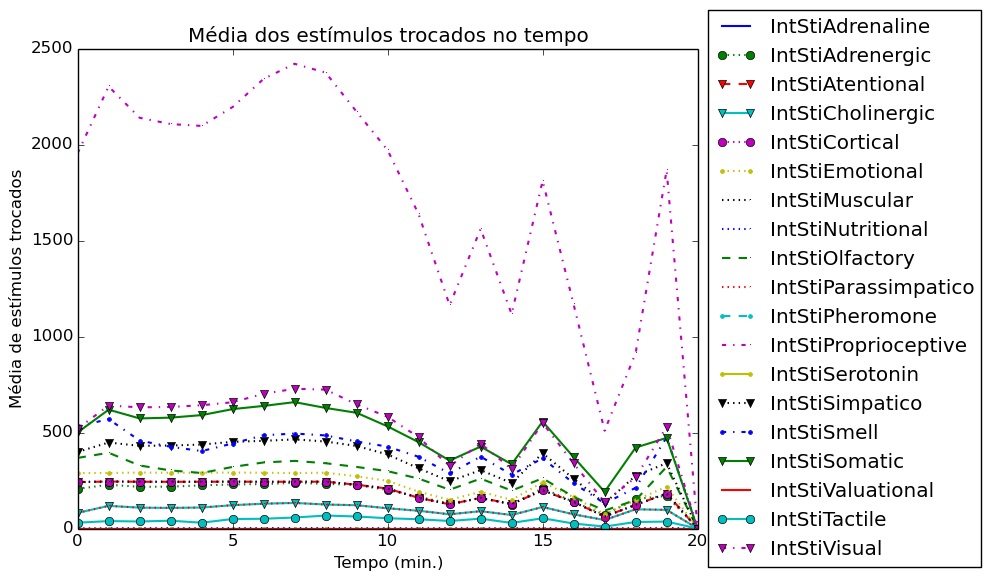
\includegraphics[width=\textwidth]{04-figuras/experiments/exp_1_artifice/avgExchangedStimuliOverTime.png}
        \label{fig:exchgStimuli_artifice}
    \end{subfigure}
    ~
    \begin{subfigure}[b]{1.0\textwidth}
        \caption{Troca de estímulos na arq. DL2L}
        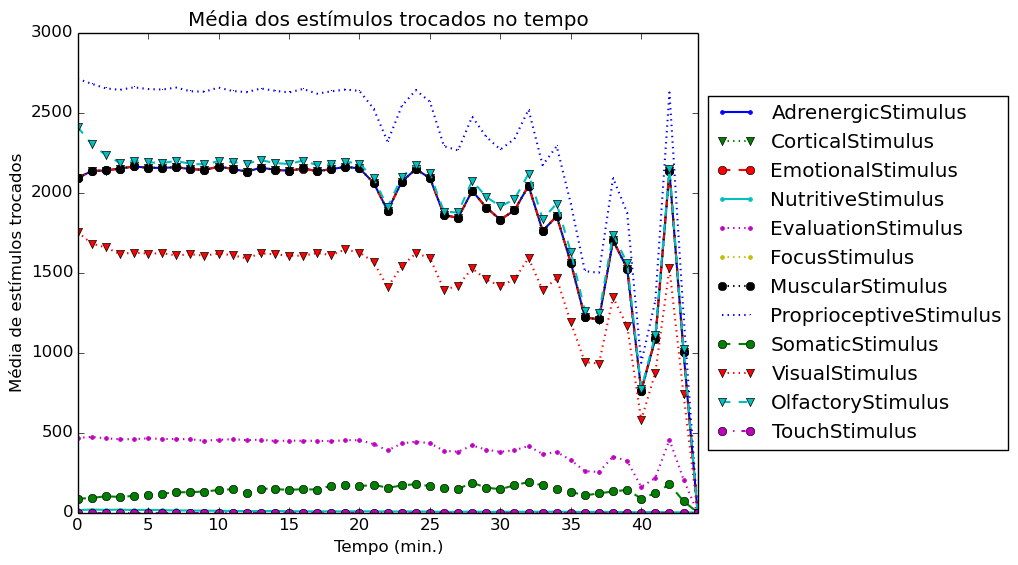
\includegraphics[width=\textwidth]{04-figuras/experiments/exp_1_l2l/avgExchangedStimuliOverTime.png}
        \label{fig:exchgStimuli_dl2l}
    \end{subfigure}
    \label{fig:exchgStimuli}
\end{figure}

A \autoref{fig:accChoices} exibe a média da soma acumulada de escolhas feitas no tempo, separadas por mecanismo. Nesta simulação foram utilizados somente os três mecanismos mais básicos: a criatura seleciona primeiro os alvos que estão à menor distância, depois seleciona a ação mais provável para cada alvo baseado na memória de condicionamento, e por fim, caso não tenha restado uma ação única, ela faz uma escolha aleatória.  

\begin{figure}[h!]
    \centering
    \caption{Gráficos da média de escolhas acumuladas no tempo para a arquitetura Artífice e DL2L}
    \begin{subfigure}[b]{1.0\textwidth}
        \caption{Arquitetura Artífice}
        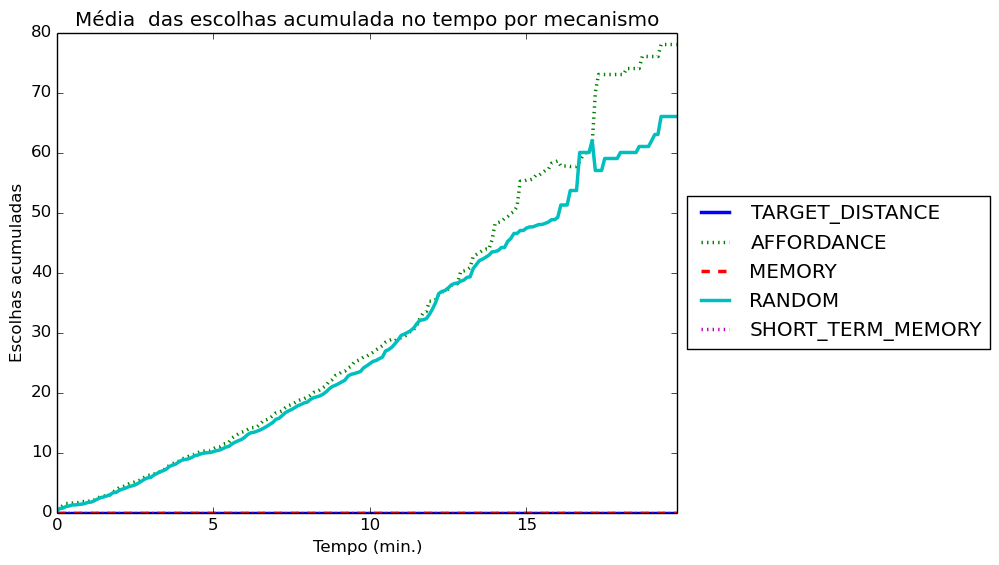
\includegraphics[width=\textwidth]{04-figuras/experiments/exp_1_artifice/accumulatedChoices.png}
        \label{fig:accChoices_artifice}
    \end{subfigure}
    ~
    \begin{subfigure}[b]{1.0\textwidth}
        \caption{Arquitetura DL2L}
        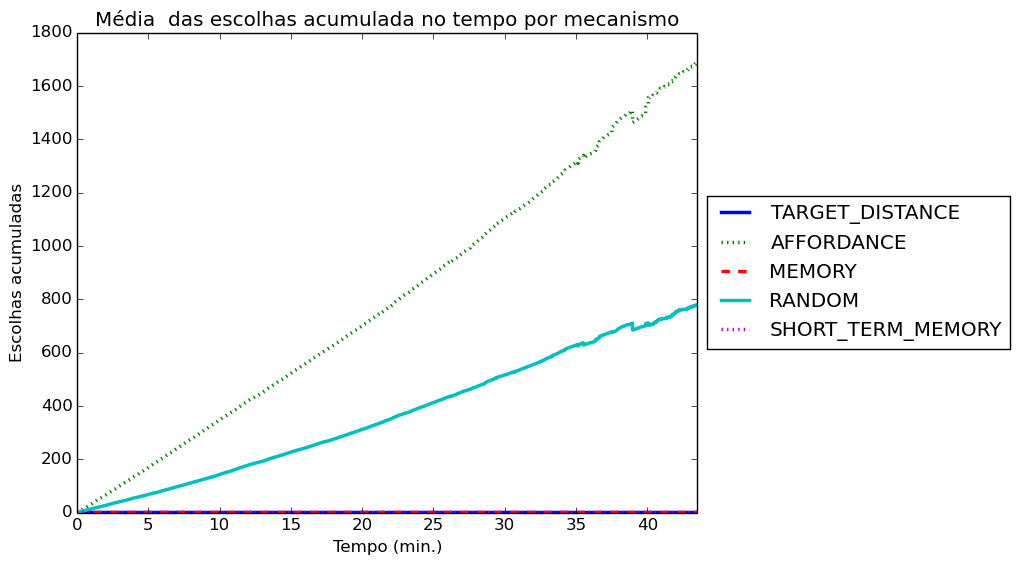
\includegraphics[width=\textwidth]{04-figuras/experiments/exp_1_l2l/accumulatedChoices.png}
        \label{fig:accChoices_dl2l}
    \end{subfigure}
  \label{fig:accChoices}
\end{figure}

A eficiência comportamental da criatura artificial é uma função do máximo \textit{arousal} e da quantidade de objetos no campo sensorial. Ela é calculada durante a execução da simulação e é utilizada para determinar a velocidade do passo da criatura e o foco atencional. Existem duas fórmulas para a eficiência comportamental, uma para tarefas simples onde a decisão envolve um único objeto, e outra para tarefas complexas que envolvem mais de um objeto. A relação da eficiência comportamental em função do \textit{arousal} máximo $A$ e o número de objetos no campo sensor $N$ é apresentada na \autoref{eq:behEfficiency}. A \autoref{fig:behEfficiency} exibe a média temporal normalizada da eficiência comportamental para as duas arquiteturas.

\begin{figure}[H]
    \caption{Cálculo da eficiência comportamental, de acordo com \citeonline{Mapa2009}}
    \[BE(A,N) = 
    \begin{cases}
        5.56A & \text{se } 0 < A < 0.18\\
        16 - 16e^{-0.4A} & \text{se } N < 2\\
        5.714A -  0.816A^2 & \text{se } N \geq 2
    \end{cases}\]
    \label{eq:behEfficiency}
\end{figure}

Para cada tipo diferente de presa a cada instante é calculado quantos nutrientes daquele tipo foram comidos, e a partir dessa série é calculada a soma acumulada. Este dado está apresentado na \autoref{fig:accNutrients} para ambas as arquiteturas.

\begin{figure}
     \centering
    \caption{Gráficos da média da eficiência comportamental no tempo para a arquitetura Artífice e DL2L}
    \begin{subfigure}[b]{1.0\textwidth}
        \caption{Arquitetura Artífice}
        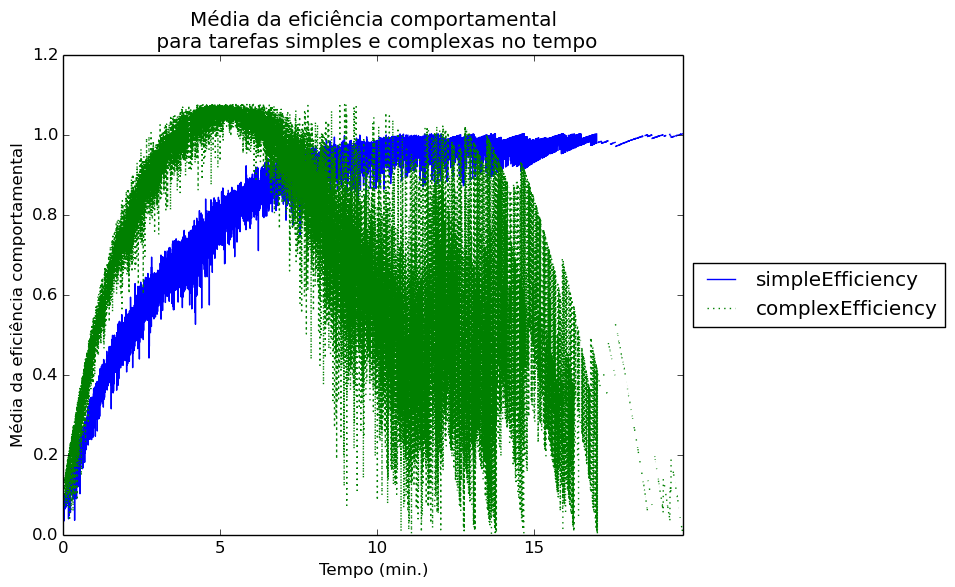
\includegraphics[width=\textwidth]{04-figuras/experiments/exp_1_artifice/behaviouralEfficiency.png}
        \label{fig:behEfficiency_artifice}
    \end{subfigure}
    ~
    \begin{subfigure}[b]{1.0\textwidth}
        \caption{Arquitetura DL2L}
        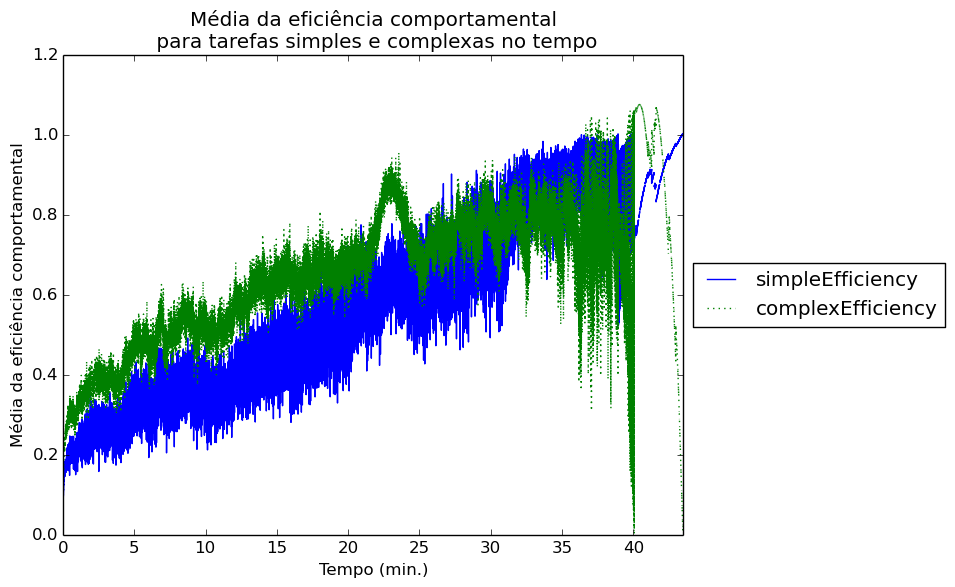
\includegraphics[width=\textwidth]{04-figuras/experiments/exp_1_l2l/behaviouralEfficiency.png}
        \label{fig:behEfficiency_dl2l}
    \end{subfigure}
    \label{fig:behEfficiency}
\end{figure}


\begin{figure}
    \centering
    \caption{Gráficos da média da soma acumulada de nutrientes comidos no tempo}
    \begin{subfigure}[b]{1.0\textwidth}
        \caption{Arquitetura Artífice}
        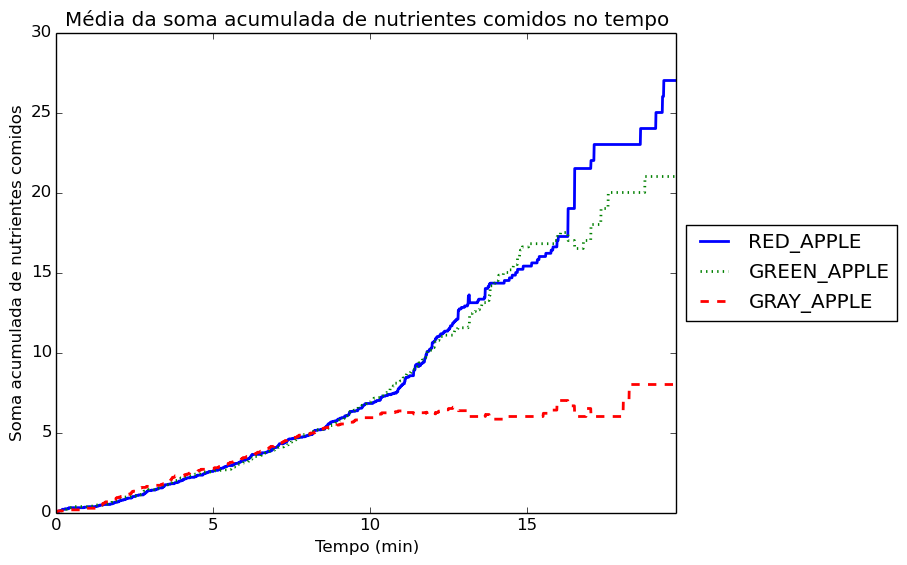
\includegraphics[width=\textwidth]{04-figuras/experiments/exp_1_artifice/accumulatedNutrients.png}
        \label{fig:accNutrients_artifice}
    \end{subfigure}
    ~
    \begin{subfigure}[b]{1.0\textwidth}
        \caption{Arquitetura DL2L}
        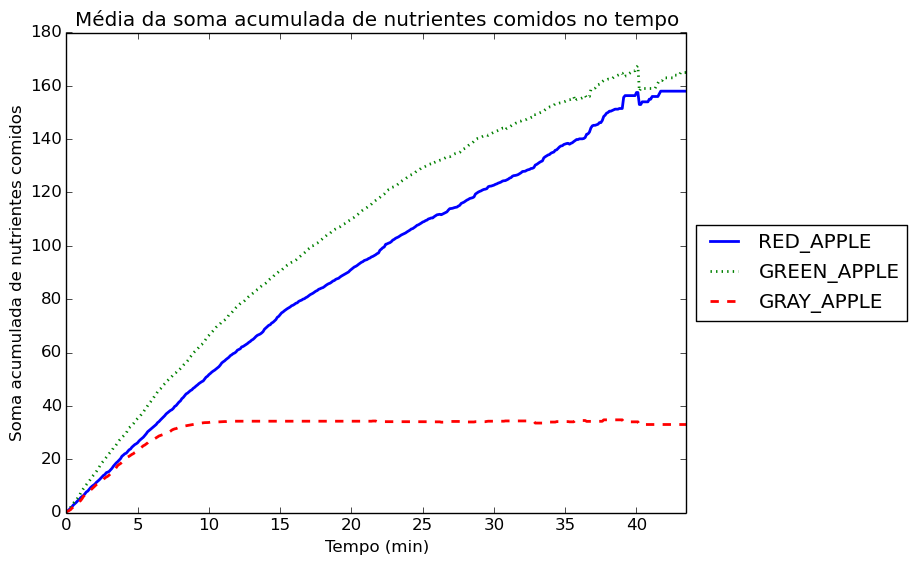
\includegraphics[width=\textwidth]{04-figuras/experiments/exp_1_l2l/accumulatedNutrients.png}
        \label{fig:accNutrients_dl2l}
    \end{subfigure}
    \label{fig:accNutrients}
\end{figure}

\section{Escalabilidade vertical}
\label{sec:esc_vertical}

A fim de verificar a influência de mais de uma criatura em um mesmo \textit{holder} na arquitetura DL2L, este segundo experimento foi proposto.  Foram executadas cinco configurações diferentes, variando o número de criaturas de 1 a 5 mantendo um único nó na simulação. A densidade do mundo é mantida constante entre as configurações, iniciando em 50 presas de cada tipo (assim como no experimento anterior) em um mundo de $4.8 \times 10^{5}$ pixeis. Cada configuração é repetida 30 vezes para garantir um erro relativo próximo a $10\%$. 

A \autoref{tab:resumo_exp2} expõe os resultados da média de tempo de vida, distância percorrida e nutrientes comidos. O erro foi calculado de acordo com a \autoref{eq:erroRelativo}.

\begin{table}[H]
\centering
\caption{Média do tempo de vida, distância percorrida e nutrientes comidos para o experimento 2}
\begin{tabular}{ccccccc}
\hline
\multirow{2}{*}{Criaturas} & \multicolumn{2}{c}{ Tempo de vida } & \multicolumn{2}{c}{ Distância percorrida } & \multicolumn{2}{c}{ Nutrientes comidos } \\
& Média & ER (\%) & Média & ER (\%) & Média & ER (\%) \\
\hline
1 & 31.40 & 6.79 & 2.72E+05 & 9.33 & 304.20 & 4.35 \\
2 & 21.71 & 8.43 & 1.83E+05 & 10.39 & 189.82 & 7.61 \\
3 & 18.81 & 7.24 & 1.30E+05 & 9.90 & 115.38 & 7.79 \\
4 & 13.51 & 6.99 & 9.59E+04 & 9.20 & 62.73 & 8.77 \\
5 & 10.38 & 4.73 & 5.43E+04 & 7.39 & 31.24 & 8.97 \\
\hline
\end{tabular}
\label{tab:resumo_exp2}
\end{table}

Os resultados para a média de estímulos trocados no tempo para cada configuração estão apresentados nas Figuras \ref{fig:exchgStimuli_dl2l}, \ref{fig:exp_2_2_exchgStimuli}, \ref{fig:exp_2_3_exchgStimuli}, \ref{fig:exp_2_4_exchgStimuli} e \ref{fig:exp_2_5_exchgStimuli}. Os gráficos para a evolução do erro relativo no tempo estão apresentados no \autoref{ap:erroExp2}.

\begin{figure}[H]
  \centering
  \caption{Média temporal dos estímulos trocados em simulação utilizando 2 criaturas}
  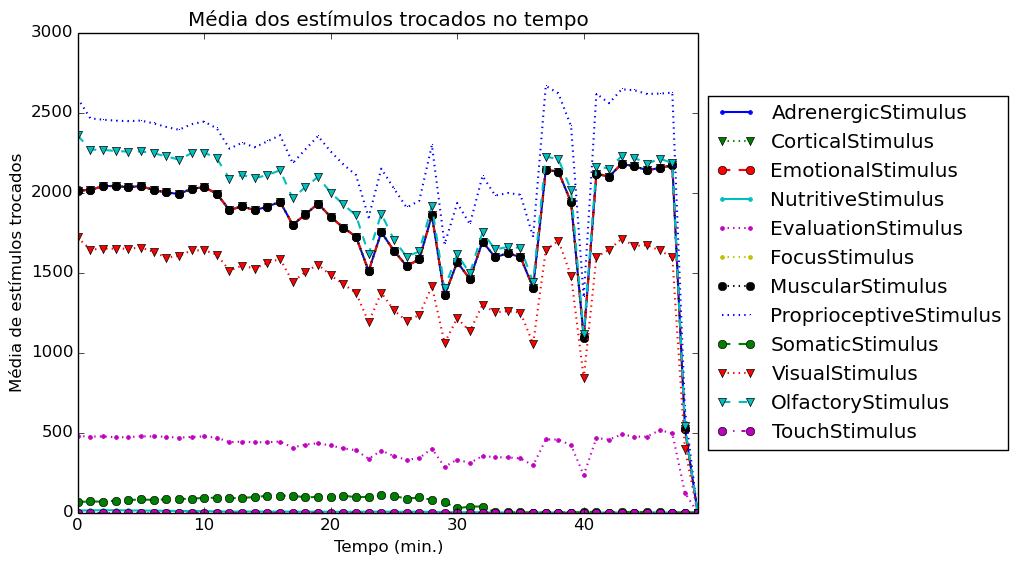
\includegraphics[scale=0.6]{04-figuras/experiments/exp_2/2/avgExchangedStimuliOverTime.png} 
  \label{fig:exp_2_2_exchgStimuli}
\end{figure}

\begin{figure}[H]
  \centering
  \caption{Média temporal dos estímulos trocados em simulação utilizando 3 criaturas}
  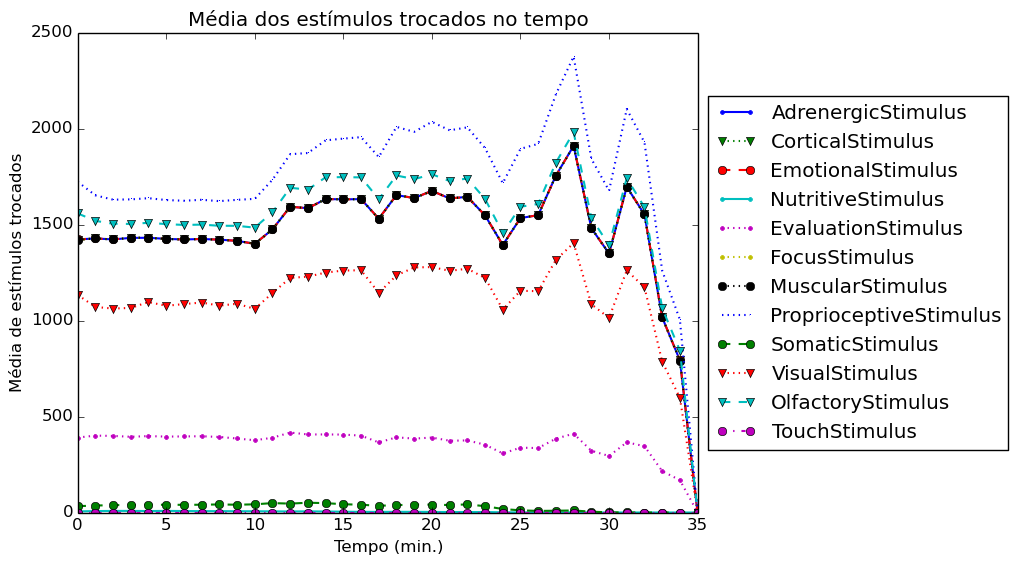
\includegraphics[scale=0.6]{04-figuras/experiments/exp_2/3/avgExchangedStimuliOverTime.png}
  \label{fig:exp_2_3_exchgStimuli}
\end{figure}

\begin{figure}[H]
  \centering
  \caption{Média temporal dos estímulos trocados em simulação utilizando 4 criaturas}
  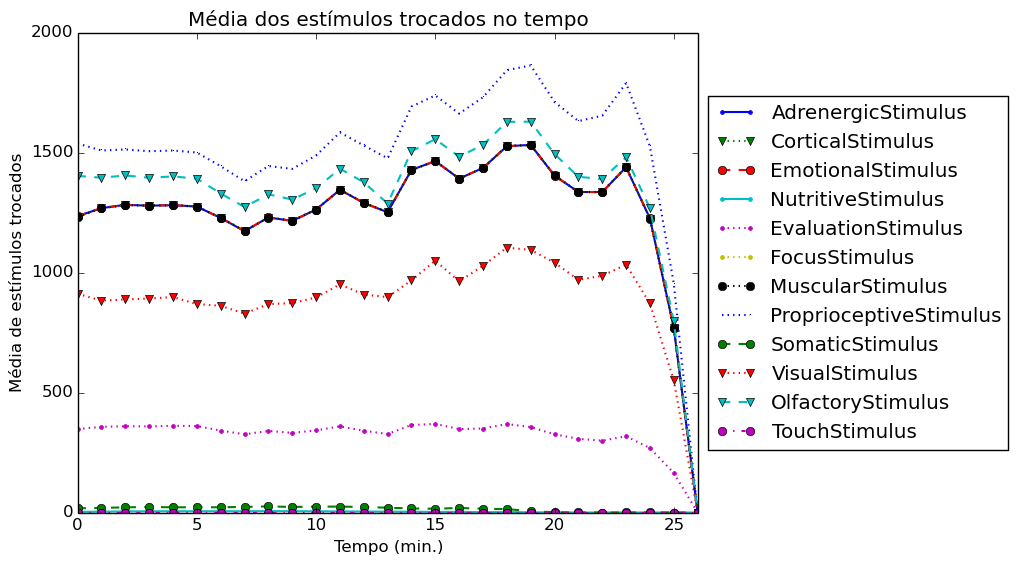
\includegraphics[scale=0.6]{04-figuras/experiments/exp_2/4/avgExchangedStimuliOverTime.png}
  \label{fig:exp_2_4_exchgStimuli}
\end{figure}

\begin{figure}[H]
  \centering
  \caption{Média temporal dos estímulos trocados em simulação utilizando 5 criaturas}
  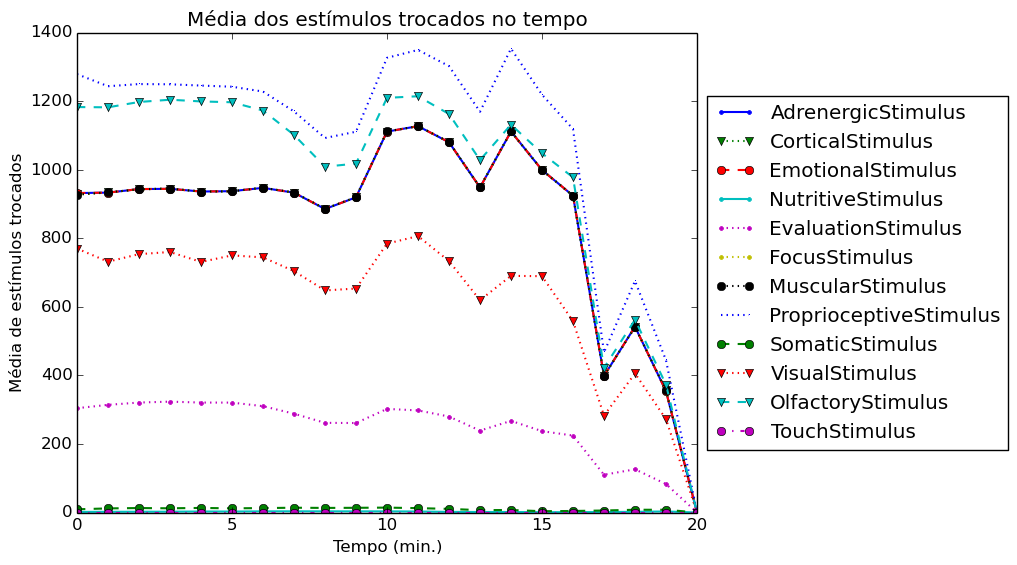
\includegraphics[scale=0.6]{04-figuras/experiments/exp_2/5/avgExchangedStimuliOverTime.png}
  \label{fig:exp_2_5_exchgStimuli}
\end{figure}

A medida que o tempo evolui o erro relativo das médias cresce. Os gráficos de erro estão apresentados na \autoref{ap:erroExp2}.

\section{Escalabilidade horizontal}
\label{sec:esc_horizontal}

Este experimento foi executado com intuito de verificar a influência de mais de um \textit{holder} em uma simulação de forrageamento. Foram executadas cinco configurações diferentes, começando com um \textit{holder} até cinco. Foi mantido o número de uma criatura por nó, e a densidade do mundo foi mantida constante, iniciando com 50 nutrientes de cada tipo em um mundo de $4.8 \times 10^{5}$ pixeis.

Na \autoref{tab:resumo_exp3} estão apresentados os resultados da média de tempo de vida, distância percorrida e nutrientes comidos. O erro foi calculado de acordo com a \autoref{eq:erroRelativo}. É notável que a medida que o número de holders aumenta, há uma diminuiçao em todas as médias. 

\begin{table}[H]
\centering
\caption{Média do tempo de vida, distância percorrida e nutrientes comidos para o experimento 3}
\begin{tabular}{ccccccc}
\hline
\multirow{2}{*}{Criaturas} & \multicolumn{2}{c}{ Tempo de vida (min.) } & \multicolumn{2}{c}{ Distância percorrida } & \multicolumn{2}{c}{ Nutrientes comidos } \\
& Média & Erro (\%) & Média & Erro (\%) & Média & Erro (\%) \\
\hline
1 & 31.40 & 6.79 & 2.72E+05 & 9.33 & 304.20 & 4.35 \\
2 & 24.69 & 8.69 & 2.24E+05 & 11.27 & 229.36 & 7.03 \\
3 & 16.85 & 6.74 & 1.64E+05 & 7.31 & 121.67 & 6.21 \\
4 & 6.75 & 5.93 & 7.06E+04 & 6.63 & 38.03 & 6.60 \\
5 & 4.82 & 3.75 & 4.93E+04 & 4.41 & 15.83 & 7.44 \\
\hline
\end{tabular}
\label{tab:resumo_exp3}
\end{table}

Dos resultados da dinâmica interna não houve alteração significativa, com exeção da média de estimulos trocados no tempo. Para cada experimento estão apresentados os resultados abaixo, salvo o experimento com um holder, cujo resultado é o mesmo apresentado na \autoref{fig:exchgStimuli_dl2l}.
\begin{figure}[H]
  \centering
  \caption{Média temporal dos estímulos trocados em simulação utilizando 2 \textit{holders}}
  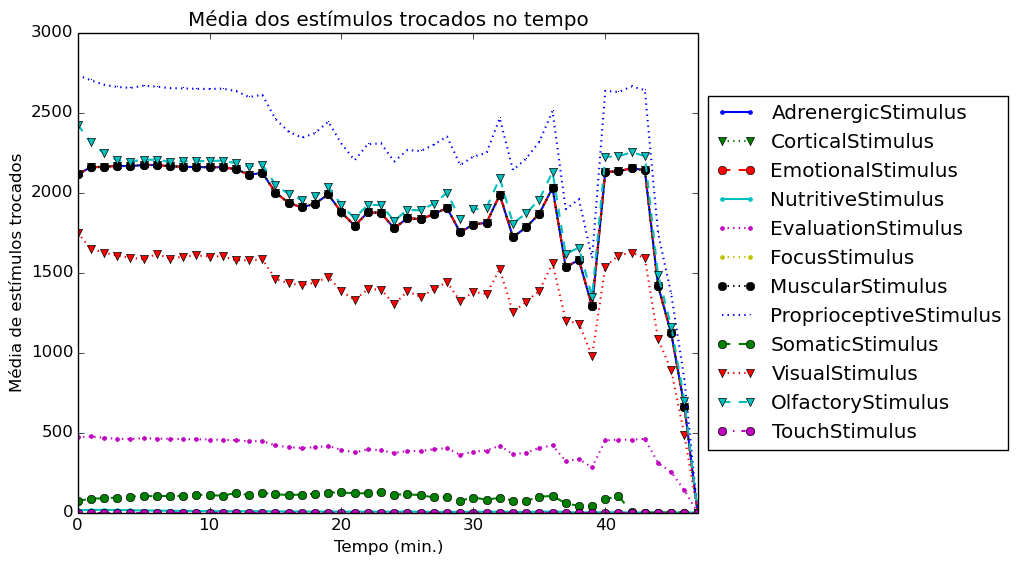
\includegraphics[scale=0.6]{04-figuras/experiments/exp_3/2/avgExchangedStimuliOverTime.png}
  \label{fig:exp_3_2_exchgStimuli}
\end{figure}

\begin{figure}[H]
  \centering
  \caption{Média temporal dos estímulos trocados em simulação utilizando 3 \textit{holders}}
  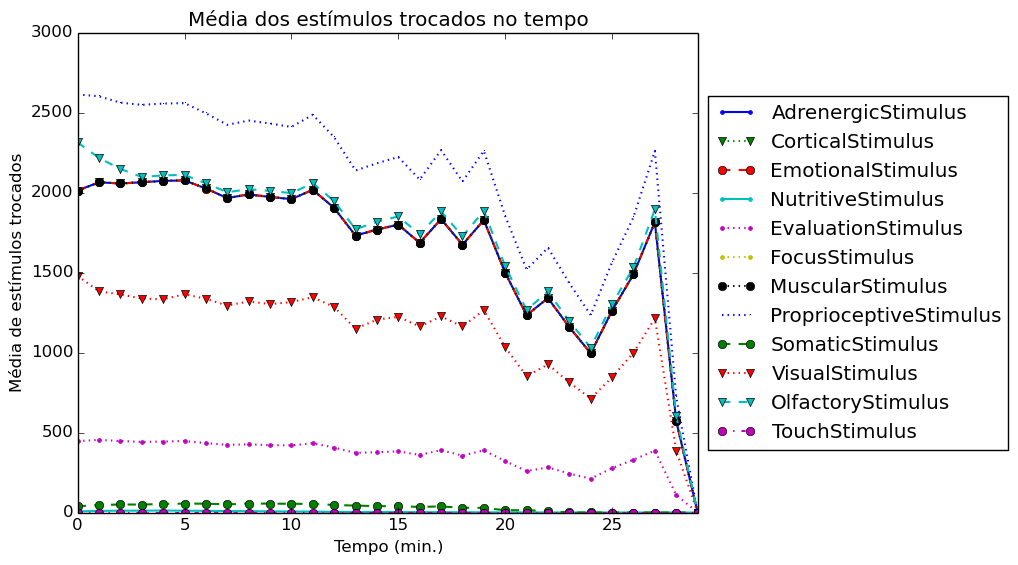
\includegraphics[scale=0.6]{04-figuras/experiments/exp_3/3/avgExchangedStimuliOverTime.png}
  \label{fig:exp_3_3_exchgStimuli}
\end{figure}

\begin{figure}[H]
  \centering
  \caption{Média temporal dos estímulos trocados em simulação utilizando 4 \textit{holders}}
  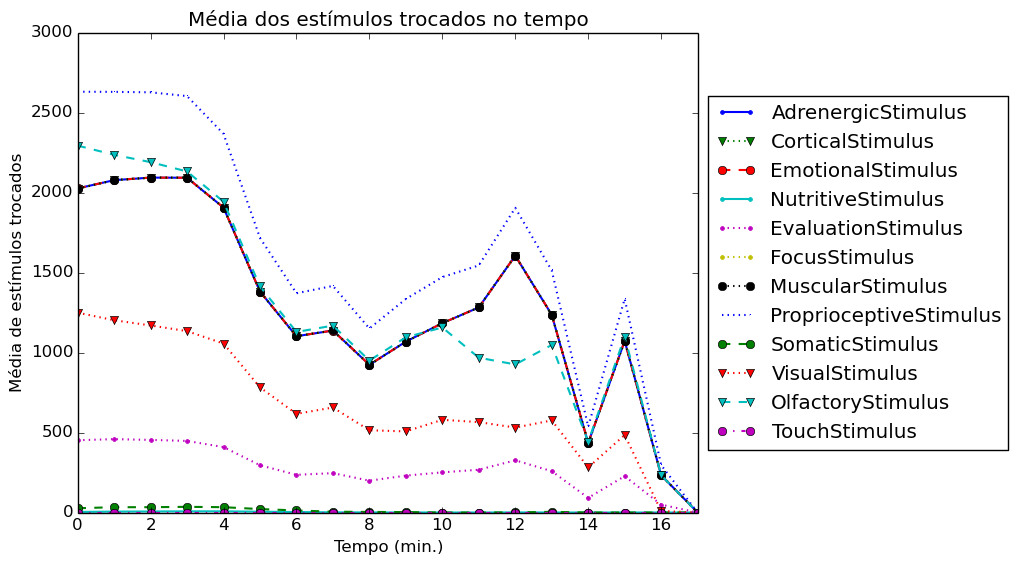
\includegraphics[scale=0.6]{04-figuras/experiments/exp_3/4/avgExchangedStimuliOverTime.png}
  \label{fig:exp_3_4_exchgStimuli}
\end{figure}

\begin{figure}[H]
  \centering
  \caption{Média temporal dos estímulos trocados em simulação utilizando 5 \textit{holders}}
  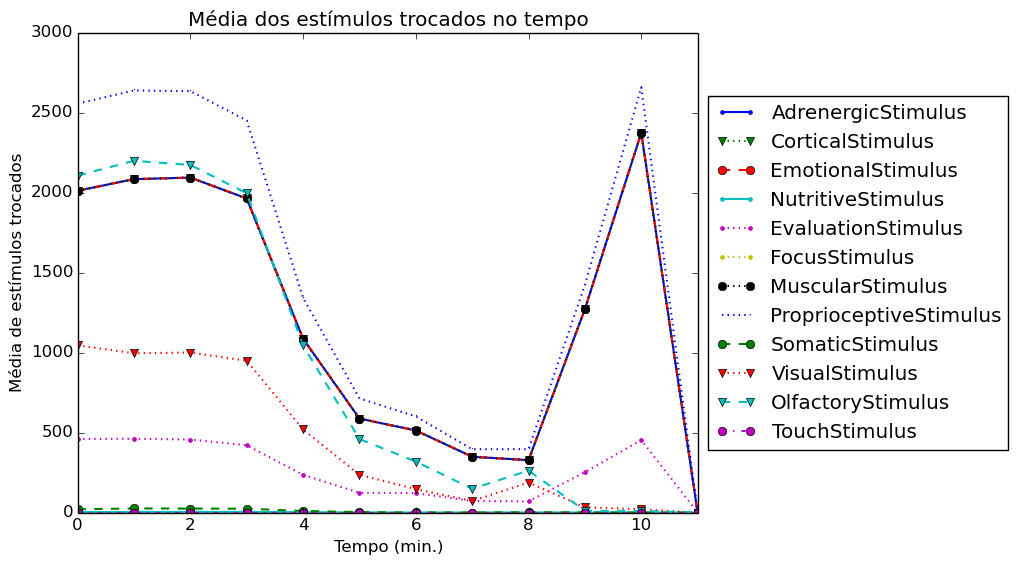
\includegraphics[scale=0.6]{04-figuras/experiments/exp_3/5/avgExchangedStimuliOverTime.png}
  \label{fig:exp_3_5_exchgStimuli}
\end{figure}

A medida que o tempo evolui e as criaturas morrem o erro relativo aumenta, e os dados próximos ao final do eixo temporal não tem confiabilidade estatística. Os gráficos da evolução do erro relativo no tempo estão apresentados na \autoref{ap:erroExp3}.

\section{Síntese dos resultados}
\label{sec:sintese}

%% exp 1
A respeito do primeiro experimento, não é possível fazer uma comparação quantitativa entre as duas arquiteturas pois ambas foram configuradas com o $\Delta_{sym}$ diferentes. Esse parâmetro exerce forte influência na dinâmica interna das criaturas e uma alteração da ordem de centésimos pode aumentar o tempo de vida em dias.  Assim, ele foi calibrado de modo que o tempo de execução das simulações fosse de no máximo uma hora, tempo que pareceu aceitável para observar o comportamento do sistema.  Entretanto o Artífice e DL2L são qualitativamente semelhantes, principalmente no que diz respeito a dinâmica interna das criaturas. Por exemplo, na \autoref{fig:accNutrients} é possível notar uma tendência semelhante na escolha de nutrientes. Ambas as arquiteturas começam escolhendo nutrientes a uma tendência parecida, quando o Artífice, por volta dos 10 minutos (\autoref{fig:accNutrients_artifice}) tem uma redução na escolha de nutrientes do tipo GRA. Este evento acontece por volta do mesmo instante de tempo na arquitetura DL2L.

É possível observar uma variação brusca na troca de estímulos proprioceptivos da arquitetura Artífice (\autoref{fig:exchgStimuli_artifice}), o que não acontece de forma tão brusca no segundo gráfico. Junto a isso, a DL2L parece exibir um comportamento mais estável ao longo do tempo comparada a sua antecessora. Uma hipótese para esses fenômenos pode estar na alocação dos componentes nas duas arquiteturas, que acontece de modo diferente. No Artífice uma \textit{thread} é escalonada para tratar estímulos, caso ela não encontre nenhum no \textit{pool} compartilhado ela entra em estado de espera até ser notificiada novamente, trata os estímulos, e entra em estado de espera por um tempo $T$ que varia de componente para componente. Essa \textit{thread} pode ser acordada após o período de espera ou durante ele (o que é chamado de \textit{spurious wakeup}), fazendo com que a execução de um componente possa vir de vários fluxos diferentes, e não necessariamente haverá estímulo para ser tratado. Por outro lado, o \textit{toolkit} Akka garante que um ator só é escalonado na presença de mensagens.

No uso dos mecanismos de escolha há uma discrepância entre as arquiteturas, enquanto na \autoref{fig:accChoices_artifice} as escolhas aleatórias praticamente acompanham as escolhas por \textit{affordances}, na \autoref{fig:accChoices_dl2l} as escolhas aleatórias estabilizam muito abaixo do outro mecanismo. Para explicar esse comportamento pode-se levantar uma hipótese sobre a velocidade e quantidade de estímulos que são recebidos e tratados pelos componentes simultaneamente. No Artífice, os componentes do sistema nervoso são escalonados para tratar estímulos à uma taxa fixa, o que leva a uma acumulação de estímulos no \textit{buffer} compartilhado por eles. Já a arquitetura DL2L tem um caráter reativo, \textit{i.e.}, os componentes reagem somente na presença de estímulo, que não tem uma frequência fixa, com exceção dos estímulos enviados pelo \textit{PartialAppraisal}. Portanto, tão logo um componente recebe um estímulo, ele é escalonado para tratá-lo. Isso diminui o número de estímulos simultâneos, o que reduz o número de \textit{affordances} que a criatura precisa escolher possibilitando uma desambiguação mais efetiva, diminuindo o número de escolhas aleatórias. 

Há uma diferença na eficiência comportamental apresentada na \autoref{fig:behEfficiency} entre as duas arquiteturas. Na \autoref{fig:behEfficiency_artifice} as curvas de tarefa simples e complexas exibem um comportamento mais semelhante ao esperado pelo cálculo da equação descrita na \autoref{eq:behEfficiency}. A \autoref{fig:behEfficiency_dl2l} exibe um comportamento médio aparentemente linear entre os minutos 0 e 31, que precisa ser melhor investigado. Mas a hipótese inicial é de que esse efeito seja somente prolongamento do eixo do tempo.

% exp 2
A partir dos resultados do segundo experimento (\autoref{tab:resumo_exp2}) pode-se observar uma diminuição do tempo de vida, da distância percorrida, e do número de presas comidas. Pelos gráficos da média de estímulos trocados no tempo (Figuras \ref{fig:exchgStimuli_dl2l}, \ref{fig:exp_2_2_exchgStimuli}, \ref{fig:exp_2_3_exchgStimuli}, \ref{fig:exp_2_4_exchgStimuli} e \ref{fig:exp_2_5_exchgStimuli}) é possível observar também uma diminuição de praticamente todos os tipos de estímulos. Posto que a densidade do mundo permanece constante, há reposição de nutrientes durante a simulação, as criaturas não interagem entre sí e por isso são independentes, e a configuração das máquinas é a mesma para todas as simulações, a única mudança entre as configurações é a quantidade de atores que executam sobre a mesma máquina. 

Partindo destes fatos e de que o componente \textit{PartialAppraisal} do SNC é o único componente que funciona à uma taxa fixa e é responsável por manter o metabolismo da criatura em funcionamento, é possível formular a seguinte hipótese sobre a diminuição do tempo de vida e o arrefecimento da troca de estímulos: os componentes são escalonados com uma menor frequência, tratando um número menor de estímulos, não havendo tempo hábil para que o sistema nervoso equilibre a dinâmica interna, levando as criaturas ao óbito mais rapidamente. Um segundo fator que provavelmente influencia na diminuição do tempo de vida médio da simulação é a sobrecarga do detector de colisões, que tem que tratar e enviar um número maior de mensagens, o que aumenta a latência entre a criatura atualizar sua posição no colisor e receber suas novas colisões.

% exp 3
No terceiro experimento é possível observar um fenômeno semelhante ao do segundo: as médias de tempo de vida, nutrientes comidos e distância percorrida diminuem a medida que aumenta o número de \textit{holders} (\autoref{tab:resumo_exp3}). Especialmente nas últimas configurações o tempo de vida diminui drasticamente comparado ao experimento anterior. Ao olhar para a troca de estímulos ao longo do tempo (Figuras \ref{fig:exchgStimuli_dl2l}, \ref{fig:exp_3_2_exchgStimuli}, \ref{fig:exp_3_3_exchgStimuli}, \ref{fig:exp_3_4_exchgStimuli} e \ref{fig:exp_3_5_exchgStimuli}) não há evidência qualitativa de que a maioria deles está diminuindo, salvo os estímulos visuais. Como as criaturas não competem por recursos na mesma máquina, só há o gargalo do detector de colisões, o que explica a diminuição desses estímulos. Como o ritmo da dinâmica continua o mesmo, somente a percepção do mundo fica mais lenta, é natural que as criaturas morram mais rapidamente.

Como dito antes, os resultados descritos acima foram preliminares e permitem apenas levantar algumas hipóteses sobre o funcionamento da DL2L. Para validar as hipóteses levantadas é necessário propor um novo conjunto de experimentos. Adiante, segue a conclusão deste trabalho, que retomará os objetivos iniciais, as principais contribuições e apontará trabalhos futuros.

